\documentclass{article}
\usepackage{sheaf-style}

\title{Assessing Model Fitness using Sheaves}
\author{Brittany Terese Fasy, Ryan Hansen, Anna Schenfisch, Daniel Salinas
Duron}

\begin{document}
\maketitle

\abstract{The purpose of science is to generate methods to predict outcomes of
events. When considering large systems with many parameters, predictions are
often subject to high variation and are subsequently hard to verify. This study
attempts to address this problem, in particular focusing on metabolism.  The
analysis showed \brittany{what analysis?} the accepted model of metabolism has
a natural representation as a $\mathit{sheaf}$ of sensor data. We find this
representation grants us three useful analytic tools.  First, it is possible to
quantify how well the model corresponds to measured data. Second, using an
iterative process called a $\mathit{consistency}$ $\mathit{radius}$
$\mathit{filtration}$, we show \todo{it is} possible to determine which
components of the model are responsible for the highest variation. We note
these components may not be an accurate representation of the process being
modeled.  Third, we build a method (finding the nearest global section) that
constructs a new model that minimizes local error for the input data. We
propose this new model is better for the given data than the previous model.}


%%%%%%%%%%%%%%%%%%%%%%%%%%%%%%%%%%%%%%%%%%%%%%%%%
\section{Introduction}
%%%%%%%%%%%%%%%%%%%%%%%%%%%%%%%%%%%%%%%%%%%%%%%%%


Sheaves are powerful tools for the integration of data of heterogeneous sources
or models\cite{robinson2017sheaves}. As such, they are useful in the
interpretation of biological data, which is often harvested from differing
populations, individuals, tissues, and cells. Our research aims to apply
sheaves in the study of metabolomics data whose inherent variability comes from
differing sources, whether the samples are obtained from different cells from
the same individual, different individuals, or both. We aim to use sheaves to
identify a consensus metabolic response to stimulus, and we aim to use that
consensus response to identify the parts of a model that do not conform to the
data.

We begin by describing the category in the domain of the sheaf, the category of
reactions, $\mathcal{X}$.  Then, we describe a mapping from the objects and
morphisms of $\mathcal{X}$ into the category in the image of the sheaf functor,
which we denote by $S$, a category of real Euclidean spaces. Finally, we define
a consistency structure on $\sheaf$ and describe how the structure can be used
in applications.

\todo{this intro is just some notes, and likely needs to be reorganized +
extended. Outline:
\begin{enumerate}
	\item \S 1 Motivation. We are using sheaves to deal with noisy data
	Consistency allows us to identify data that agree with each other.
	Identifying these has two benefits: data that agree help us identify
	metabolic profiles consistent with what we're studying, and identifying
	inconsistent data may point to parts of the model that need to be
	revised. (Model needs to be revised when data is consistent between
	samples but not when integrated with the rest of data.)
	\item \S 2  Definitions Define a sheaf, consistency radius.
	\item \S 3 Application Define a metabolic sheaf.
	\item \S 4 Experiments: Synthetic data. (possibly simulate multiple
	donors).
	\item  \S 5 Discussion
\end{enumerate}

}

%%%%%%%%%%%%%%%%%%%%%%%%%%%%%%%%%%%%%%%%%%%%%%%%%
\section{Background}
%%%%%%%%%%%%%%%%%%%%%%%%%%%%%%%%%%%%%%%%%%%%%%%%%


We begin with some necessary background and definitions from category theory.
We note that category theory was developed in the study of algebraic topology
and is typically presented in this context \cite{hatcher2002algebraic,
mac2013categories}. However, due to its wide applicability, introductions have
been developed strictly for scientific, engineering, and programming contexts
\cite{spivak2014category, fong2018seven, pierce1991basic}.  The essentials
follow below.

\definition[Category]
\label{categoryDef} 
A \emph{category} consists of three parts: (1)
objects,~(2)~morphisms between objects, and (3) a composition function that is
associative and merges two morphisms into one. A morphism is a directed
relationship between two objects in the category and is commonly represented as
an arrow from a source object to a destination object. Often, the objects in
the category give these arrows meaning. For example, in a category where the
objects are sets, there might be arrows from all subsets to their supersets, so
the arrows mean ``is a subset of''. Multiple arrows may exist between the same
pair of objects, and the identity morphism, from an object to itself, must be
included for all objects in the category. Finally, for any pair of composable
morphisms $f: U \rightarrow V$ and $g : V \rightarrow W$, their composition $ g
\circ f : U \rightarrow W $ must also be included as a morphism in the
category.

\definition[Functor] A \emph{functor} is a mapping between categories, such
that an object from the domain category has the image of some object in the
co-domain category, and morphisms also have an image morphism under the
functor. In other words, if $F: \mathcal{X} \to \mathcal{Y}$ is a functor
mapping the category $\mathcal{X}$ into the category $\mathcal{Y}$, for any
object $x \in \mathcal{X}$, $F(x)$ is an object of $\mathcal{Y}$. Also, for any
morphism between objects of $\mathcal{X}$, $f: x \to x'$, we define the image
of $f$ in $\mathcal{Y}$ as $F(f) : F(x) \to F(x')$. Note that this morphism
must already exist in $\mathcal{Y}$ for $F$ to be defined. In some cases, it is
relevant to consider a mapping that reverses all morphisms, i.e. $F(f)$ would
be defined as $F(f): F(x) \leftarrow F(x')$.  These are still considered
functors, but are referred to as \emph{contravariant} functors.  Conceptually,
contravariant functors are not distinct from ordinary functors. The reason is
that if the morphisms of any category $\mathcal{X}$ are reversed, the result is
still a category. This ``opposite'' category is denoted $\mathcal{X}^{op}$.
All contravariant functors $F : \mathcal{X} \rightarrow \mathcal{Y}$ may be
considered ordinary functors $F : \mathcal{X}^{op} \rightarrow {Y}$. Functors
are qualified as contravariant for the sake of discussing them in the context
of $\mathcal{X}$, where $\mathcal{X}$ is more germane than $\mathcal{X}^{op}$.

\definition[Sheaf] \label{sheafDef} A sheaf is a special kind of contravariant
functor. We discuss this terminology in more detail in the final pages of this
report.  In addition to being a contravariant functor, sheaves satisfy the
\emph{sheaf axioms}, which are defined in terms of objects in the domain
category and their covering families. The domain of a sheaf must therefore be a
small category equipped with a coverage. We refer the reader to
\cite{nlab:sheaf} for a discussion of coverage and smallness from a purely
categorical perspective. In this work, we only consider sheaves whose domain
categories have the following conditions: (1) the objects are the open sets of
a topological space, (2) there exists a morphism $f : U \rightarrow V$ if $U
\subseteq V$, and (3) the composition function is captured by the transitivity
of the subset relation. A covering family of an open set $U$ in this domain
category is a collection of proper subsets of $U$ whose union equals $U$. This
type of domain category category is also small; for conciseness, we will not
include justification here beyond noting that the collections of objects and
morphisms of this category type are both sets themselves. 

The sheaf axioms also impose conditions on the codomain, namely that the
objects of the codomain category are expressible as sets. The morphisms between
these sets are referred to as \emph{restrictions}. The image of an element $a
\in A$ restricted to $B$ is denoted $a |_{B}$. In this work, the objects of the
codomain category are real-valued vector spaces and the morphisms are linear
maps between them.  Real-valued vector spaces are sets and thus the sheaf
axioms can be applied. The motivation and exact definition of the sheaf in this
study can be found in \S\ref{application}.

Let $\sheaf: \mathcal{X} \rightarrow \mathcal{Y}$ be a sheaf. The sheaf axioms
are given below.
\begin{enumerate}

	\item (Locality) Let $V$ be an object in $\mathcal{X}$ and $\{U_i\}$ be
	a covering family of $V$. For any $v,v' \in \sh{V}$, if $ f_i (v) = f_j
	(v') $ for all morphisms $f_i : \sh{V} \rightarrow \sh{U_i} $, then $v
	= v'$, and

	\item (Gluing) for any open set $V$ and its covering family $\{U_i\}$,
	if there exists a union of sections $s := \bigcup_{i} (s_i \in
	\sh{U_i})$ such that, for all pairs $U_i, U_j$, $s_i |_{\sh{U_i \cap
	U_j}} = s_j|_{\sh{U_i \cap U_j}}$, then there must exist a section $v
	\in \sh{V}$ corresponding to $s$, i.e. $v|_{\sh{U_i}} = s_i$ for all
	$i$.

\end{enumerate}


%%%%%%%%%%%%%%%%%%%%%%%%%%%%%%%%%%%%%%%%%%%%%%%%%
\section{Sheaves on Systems of Linear Equations}
%%%%%%%%%%%%%%%%%%%%%%%%%%%%%%%%%%%%%%%%%%%%%%%%%

One of the most widespread techniques in modeling is to represent a system with
linear equations. Classical approaches to solving linear equations focus on
minimizing the squared sum of residuals. This is global approach minimizes a
weighted sum where each element is weighted by its own magnitude. Our approach
will find maximal partitions of equations that are self-consistent (within
partition). We describe how sheaves can provide unprecedented information on
assessing fitness of models described by systems of linear equations.


\subsection{Defining a domain category $\domain$}
\label{domainCategory}

We begin with a set, $E$, whose elements are linear equations, and a set $V$ of
the variables constrained by the equations. We use $V$ and $E$ to define the
objects of the domain category $\domain$. The objects of $\domain$ will be
open sets in a topologized partial order on $V$ and $E$. To define the partial
order, we let $V_i \leq E_j$ if $V_i$ is a term in $E_j$. To topologize, we let
the star of each element in the partial order be an open set. These initial
open sets will generate our topology. As required, we include in the open sets
any set that can be generated by the union or finite intersection of the
generators to complete the topology $\tau$.  We that note every open set $U \in
\tau$ has a subset $\eqs{U}$ of equations and a subset $\vrs{U}$ of variables.
Note, if $V_i \in V$ is a term in equations $E_p \subseteq E$, any open set $U$
that contains $V_i$ also contains $E_p$. However, the converse is not
necessarily true: if $E_p \subseteq U$, $U$ may not contain $V_i$.

Finally, we use $\tau$ to define the domain category $\domain$. We let the
objects of $\domain$, $Obj(\domain)$, be the open sets of $\tau$. We let the
morphisms be the subset relation. Explicitly, we include a morphism between
open sets $U_i$ and $U_j$ iff $U_i \subseteq U_j$.  These morphisms are
commonly referred to as \emph{inclusions} and denoted $U_i \hookrightarrow
U_j$. Finally, the transitivity of the subset relation ensures morphism
compositionality.


\subsection{Assessment Sheaf $\sheaf$}
\label{mainSheafDef}

We define sheaf $\sheaf$, a contravariant functor mapping the domain category,
$\domain$, into the codomain category, $\codomain$. The objects of $\codomain$
are solution spaces to the equations in their preimage. Recall each open set $U$
can be partitioned into variables and equations. We will refer to the variables and
equation partitions in $U$ as $V_U$ and $E_U$, respectively. 
We define $\sheaf$ formally as follows:
\begin{equation} 
 \sh{U} := \{ x | \bigwedge\limits_{E_i \in E_U} x \text{ satisfies } E_i\}.
\end{equation}
The image of $U$, $\sh{U}$, is the solution space of the system of equations
described by $E_U$.  We introduce the following notation when discussing the
image $\sh{U}$, $\eqs{U}$ refers to the equations of the preimage (this is
identical to  $E_U$), and $\vrs{U}$ refers to the set of all variables
constrained by the equations $\eqs{U}$. Thus, $V_U$ differs from $\vrs{U}$ in
that $V_U$ is the set of variables in the open set $U$ and $\vrs{U}$ are the
dimensions the solutions to $\eqs{U}$.

To complete the definition of $\sheaf$, we define the image of the morphisms in
$\domain$. Recall that morphisms in $\domain$ are inclusions $U_i
\hookrightarrow U_j$. These image of these inclusions are projections from
$\sh{U_j}$ into $\sh{U_i}$.  We formally define the projection morphism
$\sh{f}$ as follows. Let $F$ be a $n \times m$ matrix, where $m = |\vrs{U_i}|$
and $n = |\vrs{U_j}|$. Furthermore, let $v_1, ...., v_m$ be elements of
$\vrs{U_j}$. Finally, let $F_{ij} = 1$ iff $v_i \in \vrs{U_i}$ and 0 otherwise.
For all $u_i \in \sh{U_j}$, the projection of $u_i$ into $\sh{U_1}$ is defined
as
\begin{equation} 
	\sh{f}(u_i) := Fu_i.
\end{equation}
This projection maps solutions to $\eqs{U_j}$ in $\vrs{U_j}$ coordinates to solutions
to $\eqs{U_i}$ in the smaller set of coordinates $\vrs{U_i}$. For example, let
$\vrs{U_i} = \{v_1, v_2, v_3\}$, $\vrs{U_i} = \{v_1, v_2\}$, and $u_i =
\{3,6,7\}$. Then,
\begin{equation} 
F =
\begin{bmatrix}   
1 & 0 & 0 \\
0 & 1 & 0 \\
\end{bmatrix}, 
\end{equation}
and the morphism
\begin{equation}
\sh{f}(u_i) = Fu_i =  \begin{bmatrix}   
1 & 0 & 0 \\
0 & 1 & 0 \\
\end{bmatrix} \{3,6,7\}^T = 
\{3,6\}^T.
\end{equation}

Morphisms between images are well defined. Let $U_i \subseteq U_j$ be two open
sets in $\domain$. Since $U_i \subseteq U_j$, there exits an inclusion morphism
$f: U_i \hookrightarrow U_j$ between them. As a contravariant functor, $\sheaf$
defines a morphism $\sh{f} : \sh{U_j} \rightarrow \sh{U_i}$. As mentioned, the
elements in $\sh{U_i}$ are solutions to $E_{U_i}$. Thus, $\sh{f}$ maps
solutions to $\eqs{U_j}$ to solutions to $\eqs{U_i}$. Since $U_i \subseteq
U_j$, $\eqs{U_i} \subseteq \eqs{U_j}$ Therefore, elements of $\sh{U_j}$, by
satisfying  $\eqs{U_j}$, satisfy all $\eqs{U_i}$.  The morphism is thus well
defined.


\begin{theorem} 
$\sheaf$ is a sheaf.
\end{theorem}
\begin{proof} 

	We prove the theorem by establishing that $\sheaf$ is a functor whose
	image is a category satisfying the sheaf axioms, locality and gluing,
	explained in \rfdef{sheafDef}.

	\begin{lemma} $\codomain$ is a category.  \end{lemma}

      \begin{proof}

      For $\codomain$ to be a category, as elaborated in \rfdef{categoryDef},
      the objects and morphisms must be well-defined, and morphisms must be
      composable. Having defined the objects and morphisms of $\codomain$, we
      verify the compositionality of morphisms. Morphisms of $\codomain$ are
      linear transformations. Composition in $\codomain$, $\circ$, is therefore
      inherited from the compositionality of linear transformations.

      \end{proof}

	\begin{lemma} $\sheaf$ satisfies locality.  \end{lemma}

      \begin{proof}

      To prove locality, we must show that, for any open set $U$ and covering
      family $F := \{U_1, ..., U_j\}$, there cannot be two elements $s,t \in
      \sh{U}$ such that $s|_{\sh{U_i}} = t|_{\sh{U_i}}$ for all $U_i$, unless
      $s = t$.  To begin, recall that, by definition of covering family,
      $\bigcup_{U_i\in F} U_i = U$, and hence $\bigcup_{U_i \in F} \vrs{U_i} =
      \vrs{U}$.  The set $\vrs{U_i}$ must be a subset of $\vrs{U}$, since, if
      $U_i$ is a member of the covering family, the morphism $U_i
      \hookrightarrow U$, denoting inclusion,  must exist.  Hence, all $U_i$ in
      the family are subsets of $U$ and $\vrs{U_i} \subseteq \vrs{U}$.
      Elements $s,t \in \sheaf(U)$ are also elements of $\R^n$, with a
      dimension corresponding to each element in $\vrs{U}$. For any $U_i \in
      F$, $\vrs{U_i} \subseteq \vrs{U}$, and therefore $s|_{\sh{U_i}}$ has a
      subset of the coordinates of $s$, and likewise for $t$ and
      $t|_{\sh{U_i}}$. Recall, the morphism $f: \sh{U} \to \sh{U_i}$ is nothing more than 
an identity projection from $\mathbb{R}^n$ to $\mathbb{R}^m$, forgetting 
the variables from $\vrs{U}$ not included in $\vrs{U_i}$. Then when $s|_{\sh{U_i}}$ = $t|_{\sh{U_i}}$ both $s$ and $t$
      must have the same values in the coordinates corresponding to $V(U_i)$.
      If $s|_{\sh{U_i}}$ = $t|_{\sh{U_i}}$ is true for all $U_i$, then $s$ and
      $t$ must have the same value for all coordinates and $s = t$.

      \end{proof}

	\begin{lemma} $\sheaf$ satisfies gluing. \end{lemma}

      \begin{proof}

      Given an open set $U$ and a covering family $F := \{U_1, ... , U_k\}$,
      gluing requires that, for any collection $\hat{s} := \bigcup_{U_i \in F}
      (s_i \in \sh{U_i})$ such that $\forall U_i, U_j \in F$, $s_i |_{\sh{U_i
      \cap U_j}} = s_j|_{\sh{U_i \cap U_j}}$, there must exist a $s \in \sh{U}$
      such that for each $U_i \in F$, $s|U_i = s_i$.   Consider an arbitrary
      variable $v \in \vrs{U}$. Since $F$ is a covering family of $U$, we know
      $\vrs{U} = \bigcup_{U_i \in F}\vrs{U_i}$. Then $v$ must be contained in
      at least one $U_i$, and there must exist at least one $s_i$ associating a
      value to $v$. We denote the value that $s_i$ sets for $v$ as $q_i$. 

      By hypothesis, $s_i \in \sh{U_i}, s_j \in \sh{U_j}$, and $s_i|_{\sh{U_i
      \cap U_j}} = s_j|_{\sh{U_i \cap U_j}}$ for each $U_i, U_j \in F$. But
      recall, the morphism $f : \sh{U} \to \sh{U_i}$ is nothing more than an
      identity projection from some $\mathbb{R}^n$ to $\mathbb{R}^m$ for $m
      \leq n$, forgetting the variables from $\vrs{U}$ not included in
      $\vrs{U_i}$. Then, each $s_i$ containing a value for $v$ must have the
      same value $q_i$, otherwise $s_i|_{\sh{U_i \cap U_j}} \neq s_j|_{\sh{U_i
      \cap U_j}}$ for each $U_i, U_j \in F$. Since $v \in \vrs{U}$, $s$ must
      also contain a value for $v$, and to satisfy the identity morphisms of
      $\sheaf$, this value must also be $q_i$.

      Since $s$ requires exactly one value for each $v \in \vrs{U}$, by
      arbitrariness of $v \in \vrs{U}$, we can conform all of $s$ from the
      $q_i$ values of all $v$. If, for all $v$, $s$ has value $q_i$, then
      $s|_\sh{U_i} = q_i$ for each $U_i \in F$ that contains $v$, and indeed
      $s|\sh{U_i} = s_i$, as desired.

      \end{proof}

      By the Lemmas above, $\sheaf$ must therefore be a sheaf.
\end{proof}

\begin{example}
	Suppose we have a an $S_0$ with three objects.
	Let $A=\{x,y,z|3x + 2y -z = 0\}, B=\{w,x|2w-5x=0\}, C=\{x\}$, and $Obj(E_0) 
	= 
	\{A,B,C\}$. As morphisms, we identify the relationship preserving maps as 
	$hom(E_0) = f:A \to C,g:B \to C$. If $a\in A, b \in B,$ then we can write 
	$a=[a_x,a_y,a_z],b=[b_w,b_x]$. We define $f(a)$, in essence, as setting 
	specific values for its governing equation. $f(a) = \{x|3x +2a_y-a_z=0\}$ 
	and 
	$g(b)=\{x|2b_w-5x=0\}$. We hope $x$ restricts to the same value in each, as 
	that indicates that the data is consistent within our objects, and 
	furthermore when we apply our sheaf, by sheaf 
	gluing, implies that $x$ is part of a self-consistent higher order set, 
	containing $w,x,y,z$.

\end{example}

\subsection{Model Assessment}
We propose $\sheaf$ as an improved mechanism to measure consistency on linear systems.
Traditionally, linear systems are qualified as consistent based on least
 squares analysis. Least squares works by finding an approximate
 solution to a linear system that minimizes some norm (typically $L2$)
 between itself and the solution space. To illustrate, consider the following
system of linear equations and data expressed in matrix form. 
$\begin{bmatrix}
1 & 2 & 3\\
2 & 2 & 3
\end{bmatrix} \times \begin{bmatrix}
v_1 \\
 v_2 \\
 v_3
\end{bmatrix} = \begin{bmatrix}
1 \\ 
 3\\
\end{bmatrix}$
 \daniel{this is where we should outline a scenario where least squares is
inadequate. experiments should clarify.}

\definition[Sheaf assignment]

An assignment, $\phi$, is intended to integrate data and measurements
into the abstract framework provided by sheaves. Formally, an assignment can be
obtained by selecting an element from the Cartesian product of all open set
images, 
\begin{equation}
\phi \in \prod_{U \in Obj(\domain)} \sh{U} .
\end{equation}
As such, an assignment contains one element from the image of each open set $U$
in the domain category.

\definition[Consistency Structure] An assignment that contains values that are
compatible under restriction is deemed \emph{consistent}.  We define
consistency formally as follows. Given a topology $\tau$, an assignment $\phi$,
and a sheaf $\sheaf$ with domain $\tau$ as described in \S
\ref{domainCategory}-\ref{mainSheafDef}, a \emph{consistency structure} is a
set of consistency functions that output a Boolean value,
\begin{equation}
\cfn_U(\phi) \rightarrow \{0,1\},
\end{equation} 
one for each open set $U \in \tau$.\footnote{This consistency structure is
analogous to the one defined in \cite{praggastis2016maximal}, though they
differ in domain.} The function $\cfn_U$ operates on the the elements of $\phi$
corresponding to $\sh{U_i}$, where $\{U_i\}$ conform the \emph{star} of an open
set $U$ as defined in \S\ref{domainCategory}. Specifically, it is a combination
\begin{equation} 
\cfn_U(\phi) : \bigoplus_{i} \sh{U \subseteq U_i}(\phi_i) \rightarrow \{0,1\},
\end{equation}
where $\sh{U \subseteq U_i}(\phi_i)$ is the restriction of $\phi_i$ to
$\sh{U}$, and $\oplus$ is model-specific. A canonical example\footnote{ This is
referred to as the standard consistency structure in
\cite{praggastis2016maximal}.} is to let
$\oplus$ be $\wedge$ (logical \emph{and}) and 
\begin{equation} 
\cfn_U(\phi)( \sh{U \subseteq U_i}(\phi_i) )  = 
\begin{cases}  
1 & \text{if } \sh{U \subseteq U_i}(\phi_i) = \phi_U,  \text{and} \\
0 & \text{otherwise.}
\end{cases}
\end{equation}
For this consistency structure, an assignment $\phi$ is consistent iff the
restrictions of all $\phi_i$ to $\phi_U$ equal the value of  $\phi_U$.
Variations of this consistency structure might include some tolerance value
$\delta$, where 
\begin{equation}
\cfn_U(\phi)( \sh{U \subseteq U_i}(\phi_i) ) = 1 \text{ if } | \sh{U \subseteq
U_i}(\phi_i) - \phi_U  | \leq \delta.
\end{equation}
If $\cfn_U(\phi) = 1$ for all open sets $U$ in the topology $\tau$, then $\phi$ is consistent.

\subsection{Maximal Consistent Subsections}
For each $\sh{U_i}$ we look at all the incoming restriction morphisms
$\{\sh{U_j \leq U_i} | U_j \leq U_i\}$. If our consistency function
$\mathscr{C}_i$ evaluates to true, we know the stalk $\sh{U_i}$ is self
consistent within its immediate locale - the preimage of the restriction
morphisms we just dealt with will be in the same maximal consistent subsection
as the stalk. If $\mathscr{C}_i$ evaluates to false, we know the restriction
morphisms are not consistent, and therefore the stalk $\sh{U_i}$ is NOT self
consistent within its immediate locale - the preimage of the restriction
morphisms will not be included in the same maximal consistent subsection as the
stalk.

\subsubsection{Algorithm}
We start at the bottom level of $\sh{\mathscr{X}}$, the part of the sheaf with no
outgoing restriction morphisms. This corresponds to our individual metabolites.
We add each individual metabolite to its own consistent subsection , and note
at worst, each metabolite is consistent with itself only. 
 Each level, we test to see if restriction morphisms
are deemed consistent via our consistency functions, and proceed based on
their return value. If true, we add the node to the current consistent
subsection, $\sh{\Gamma_i}$. If two subsections argue over a node, we merge
the subsections. Finally, if false, we stop the algorithm on that branch.
A false value means we have determined the largest consistent subsection 
the measured metabolic data can exist on.

\subsection{Residual Analysis}
We bring attention to the standard approach for assessing consistency in
systems of linear equations - examining the size of residual error compared
to an associated expected solution. For a set of equations $E$, a set of
initial variable measurements $V$, and final measured values for the variables $M$, residual analysis
typically takes the form of a linear algebra problem. From $E$ construct
a matrix of equations $A$, from $V$ define a vector of variables $x$
representing an expected solution, and from $M$ construct 
a constant vector of measured values $b$. If an exact solution were to exist,
the equation $Ax = b$ would be true. However, to find residual error,
the technique is to find an approximate solution by solving a perturbed 
problem: $A \tilde{X} = b + \Delta b$. The residual vector is defined as $r=b-A\tilde{x}$
and geometrically is the distance from the measured values to the 
perturbed measured values in the approximate solution.


\daniel{This is motivated by the praggastis paper. The paper's central theorem
is that there exist maximal sections that are self-consistent. The preimage of
these sections are subcomplexes in an ``abstract simplicial cell complex''.
The vertices of these complexes are sensors which measure variables. There
exists a $k$-cell between $k$ sensors that share a measured variable. e.g. if
sensors $v_1$ and $v_2$ both measure $a$, then there exists an edge between
them. this is a cell complex, but it becomes a simplicial complex because when
$V := v_1, ..., v_k$ all measure $a$, any subcomplex $V' \subset V$ is also
included, satisfying the simplicial requirements. The subset relation induces a
partial order which induces the open sets using stars. The image of the open
set $V$ is the set of possible values for the variables measured, in this case
$a$.

This is comparable to what we have. Let each equation be a sensor that measures
a set of variables (metabolites) $V$. Consider the open set that is the star of
a maximal $k$ cell (the star of it is just itself). Assume that all of the
equations overlap on just a single variable (metabolite). Then this open set is
present in both the topologized simplicial complex and the topologized partial
order we defined.}


\subsubsection{Assignment}
The first step in defining consistency is to generate our original assignment, 
$(\sheaf, A)$, .
Let $m$ be a set of measured values, one measured value attributed to each 
metabolic variable, and $V(U)$ be the set of metabolic variables in an 
open set $U$. Then we designate our assignment as follows:
Take $m_v \subset m$, the subset of $m$ such that it associates exactly one 
value to each $V(U)$. Then we assign $(\sh{U}, m_v)$. Extending the same 
process to each open set
conforms $A$.

\subsubsection{Error}
Since $\sheaf$ maps to some $\mathbb{R}^n$, there is a natural pseudometric on 
the 
space of assignments. For some stalk $\sh{U}$, and two values assigned to that 
stalk, $a$ and $b$, we define the error between stalk assignments as 
$E((\sh{U},a), 
(\sh{U},b)):= 
d(a,b)$, the 
euclidean distance 
between 
the assignment values. We 
call this the \emph{error} of $\sh{U}$. Recall \emph{definition 2.8}, and 
notice minimizing error is the foundation for optimizing Consistency Radius.

\subsubsection{Consistency Radius Filtration} %\todo{Error filtration?}\\
We can compute the error on each pair of stalk assignments joined by 
restriction 
morphism. This admits a natural filtration on the error of each pair of 
assignments, where we slowly add objects that are within $\epsilon$ error of a 
given stalk. We say a 
restriction morphism $f:\sh{U_2} \to \sh{U_1}$, with corresponding assignments 
$(\sh{U_2},a_2)$ and  $(\sh{U_1},a_1)$ enters our space at time $t$ if 
$d(a_1,a_2) = t$.\\ Remark: An object entering the filtration signifies how 
well the restriction respects the assignment. In our scenario, an object 
that enters the filtration early on means the two stalks have compatible data.

 \begin{theorem}
	If a global section exists, our measured data is perfectly consistent with 
	all reaction equations.
\end{theorem}
\begin{proof}
	a little bit tougher than the last one
\end{proof}


\section{Numerical Example}
We provide a simple numerical example to demonstrate the utility of sheaf 
consistency.
We consider the following reactions and rates for our numerical example:
\begin{align}
A + 2B &\rightarrow 5C \,\,\, \text{at rate $r_1$} \\
A &\rightarrow 3B \,\,\, \text{at rate $r_2$} .
\end{align}

\subsection{Category of Reactions}

The equations governing the metabolite rates of change are
\begin{align}
	E_1: \Delta A &= -r_1 - r_2,\\
	E_2: \Delta B &= -2r_1 + 3 r_2,\\
	E_3: \Delta C &= 5r_1.
\end{align}

The corresponding partial order is defined by letting a variable $V_i \leq E_j$
if $V_i$ is a term in $E_j$. Our example has the following partial order:

\begin{figure}[h]
	\centering
	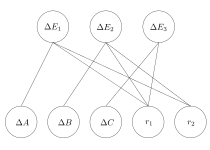
\includegraphics[width=.5\textwidth,height=.3\textwidth]{./figs/poset.pdf}
	\caption{Picture depicting partial order of equations and variables.}
\end{figure}

%	\Delta A \leq E_1, r_1 \leq E_1, r_2 \leq E_1,\\
%	\Delta B \leq E_2, r_1 \leq E_2, r_2 \leq E_2,\\
%	\Delta C \leq E_3, r_1 \leq E_3.

We endow this partial order with the upper topology, where the 
open sets of the
topology are the upper sets of each element in the partial order. We note here
that all open sets $U$ in the upper topology have the following property: if $x$
is in $U$, then the upper set of $x$, $\bigstar(x)$, is also contained in $U$.
Thus, we label our open sets using the smallest number of members whose upper
sets conform the set. For example, the open set $\{\Delta A, E_1\}$ is labeled
$U_{\bigstar(A)}$, and the open set $\{r_1, \Delta A, E_1, E_2, E_3 \}$ is
labeled $U_{\bigstar(r_1, \Delta A)}$.  Finally, we that note any open set $U$
can be partitioned into a set of variables, denoted $V_U$, and constraining
equations, denoted $E_U$. The generating open sets for the upper topology are
given below:

\begin{align}
	U_{\bigstar(\Delta A)} &:=
	E_{U_{\bigstar(\Delta A)}} \cup V_{U_{\bigstar(\Delta A)}} =
	\{E_1\} \cup \{\Delta A \} = \{E_1, \Delta A \},\\
	U_{\bigstar(\Delta B)} &:=
	E_{U_{\bigstar(\Delta B)}} \cup V_{U_{\bigstar(\Delta B)}} = 
	\{E_2\} \cup \{ \Delta B \} = \{E_2 \cup \Delta B \},\\
	U_{\bigstar(\Delta C)} &:=
	E_{U_{\bigstar(\Delta C)}} \cup V_{U_{\bigstar(\Delta C)}} =
	\{E_3\} \cup \{ \Delta C \}  = \{E_3, \Delta C \},\\
	U_{\bigstar(r_1)} &:=
	E_{U_{\bigstar(r_1)}} \cup V_{U_{\bigstar(r_1)}} =
	\{E_1,E_2,E_3\} \cup \{ r_1 \} = \{E_1,E_2,E_3, r_1 \},\\
	U_{\bigstar(r_2)} &:=
	E_{U_{\bigstar(r_2)}} \cup V_{U_{\bigstar(r_2)}} =
	\{E_1,E_2\} \cup \{ r_2 \} = \{E_1,E_2, r_2 \}, \\
	U_{\bigstar(E_1)} &:=
	E_{U_{\bigstar(E_1)}} \cup V_{U_{\bigstar(E_1)}} =
	\{E_1\} \cup \emptyset = \{E_1\}, \\
	U_{\bigstar(E_2)} &:=
	E_{U_{\bigstar(E_2)}} \cup V_{U_{\bigstar(E_2)}} =
	\{E_1\} \cup \emptyset = \{E_2\}, \\
	U_{\bigstar(E_3)} &:=
	E_{U_{\bigstar(E_3)}} \cup V_{U_{\bigstar(E_3)}} =
	\{E_3\} \cup \emptyset = \{E_3\}. \\
\end{align}

The collection of open sets of a topology is, by definition, closed under union
and finite intersection. Thus, we include any set that can be produced by the
union or intersection of these generators in the open sets.

Finally, we are ready to define the domain category, $\mathscr{C}$. The objects
of $\mathscr{C}$ are the open sets. The morphisms are inclusions, denoted with
$\hookrightarrow$. Thus, if $U_1 \subseteq U_2$, then the morphism $U_1
\hookrightarrow U_2 $ exists in the category. Transitivity of inclusion ensures
morphism compositionality.

\subsection{Category of Solutions}

We begin our definition of the category of solutions, $S := \sh{\mathscr{C}}$,
by defining objects of $S$. These are the stalks $\sh{U}$ of each open set $U$.
The stalk of  $U$ is the set of solutions to the equations in $E_U$, projected
onto the variables in  $V_U$.

For example, the stalk of generator $U_{\bigstar(\Delta A)}$ is the set of
solutions to the equations in $E_{U_{\bigstar(\Delta A)}}$ projected onto the
variables in $V_{U_{\bigstar(\Delta A)}}$. The set of solutions to
$E_{U_{\bigstar(\Delta A)}}$ is the set of solutions to $E_1$,
\begin{equation}
	\{\Delta A, r_1, r_2 \:|\: \Delta A -r_1 - r_2  = 0 \}.
\end{equation}
The set of variables in  $V_{U_{\bigstar(\Delta A)}}$ consists only of $\Delta
A$. Therefore, the stalk $\sh{U_{\bigstar(\Delta A)}}$ of $U_{\bigstar(\Delta
A)}$ is
\begin{equation}
	\{\Delta A \: | \: \Delta A -r_1 - r_2  = 0 \}.
\end{equation}
The stalk for $U_{\bigstar(\Delta A)}$ is therefore $\mathbb{R}^1$, since
$\Delta A$ is unbounded.

In general, stalks projected onto $n$ variables are not $n$-dimensional. To
explain this, we first consider a general stalk $\sh{U}$. The elements of this
stalk are the solutions the equations $E_i \in E_U$. All equations will have
the form
\begin{equation} 
E_i := \sum_{k} r_k + \Delta X  = 0,
\end{equation}
wherein they are expressed as the sum of several rates and a single change in
metabolite $X$. The equations in of $E_U$ define a system of linear equations,
typically expressed in matrix form. For example, if we let $E_U := \{E_1,
E_2\}$ in our continuing example, the matrix form would be 
\begin{equation}
\bordermatrix{
  ~  & r_1 & r_2 & \Delta A & \Delta B \cr
E_1 & 1  & 2  &  1       &  0 \cr
E_2 & 2  & -3   &  0       &  1\cr
} \begin{pmatrix} r_1 \\ r_2 \\ \Delta A \\ \Delta B \end{pmatrix} = \begin{pmatrix} 
 0 \\ 0
 \end{pmatrix}.
\end{equation}
matrix that has the stoichiometric coefficients. This quantity is at least the
number of columns of the matrix minus the number of rows. If all the rows are
linearly independent, these two quantities are equal by the fundamental theorem
of linear algebra. The rows of any $E_U$ will always be linearly independent,
since each $E_i$ corresponds to a single metabolite, which implies its row will
have a unique term. Thus, the dimension of any stalk is at most the number of
columns minus the number of rows. If $V_U$ is larger than this quantity, then
the stalk will be a subspace of its ambient space.

For example, consider the stalk $\sh{U_{\bigstar(r_1, r_2, \Delta C)}}$,
conformed of the points
\begin{equation} 
	\left\{r_1, r_2, \Delta C \: \middle| \:
	\begin{split}  
	 \Delta A + r_1 + r_2  &= 0 \\
	 \Delta B +2r_1 - 3r_2  &= 0 \\
	 \Delta C - 5r_1 &= 0
	\end{split}
	\right\}.
\label{r1r2c}
\end{equation}
The corresponding matrix is
\begin{equation} 
\bordermatrix{
~   & r_1 & r_2 & \Delta A & \Delta B & \Delta C \cr
E_1 & 1  & 2    & 1 & 0 & 0 \cr
E_2 & 2  & -3   & 0 & 1 & 0 \cr
E_3 & -5  & 0    & 0 & 0 & 1 \cr
}
\end{equation}
Thus, the solutions to the linear system in Eq.~\ref{r1r2c} lie on a
two-dimensional plane. Because we consider three variables, variables $r_1,
r_2$ and $\Delta C$, the resulting space is not $\mathbb{R}^3$.

Open sets with $n$ participating reaction variables are sent to $\mathbb{R}^n$
and inclusion morphisms are sent to restrictions, where restrictions in essence
set values of variables. The following is an example path of restrictions. We
denote an open set that contains equations $E_1, E_2$ and $V_1, V_2$ as
$U_{\{E_1,E_2,V_1,V_2\}}$.

\begin{align}
	\sh{U_{\{E_1, E_2, E_3, \Delta A, \Delta B, \Delta C, r_1, r_2\}}} \to 
	\sh{U_{\{E_1, E_2, E_3, \Delta A, \Delta B, r_1, r_2\}}} \to \sh{U_{\{E_1, 
	E_2, E_3, \Delta A, r_1, r_2\}}} \\
	\to 
	\sh{U_{\{E_1, E_2, E_3, \Delta 
	A, r_1\}}}
	\to 
	\sh{U_{\{E_1, \Delta A\}}}
\end{align}


\textbf{Assignment}\\
Suppose we are given some measured data.
\begin{align*}
\Delta A &= -10 \\
\Delta B &= 15 \\
\Delta C &= 8 \\
r_1 &= 2 \\
r_2 &= 7.
\end{align*}
We want to see if this data is consistent with our model. From \todo{Theorem 
x}, the data is consistent if and only if the assignment yields a global 
section. To do verify if this global section exists, we propagate the initial 
assignment through the entirety of $S$ by applying restriction morphisms.
Following (20), applying the measured values to restricted stalks, we get 

\begin{align*}
	\sh{U_{\{E_1, E_2, E_3, \Delta A, \Delta B, \Delta C, r_1, r_2\}}}= \\
	\{(\Delta A, \Delta B, \Delta C, r_1, r_2) \in 
	\mathbb{R}^5:\Delta A 
	+r_1+r_2=0, \Delta B+2r_1-3r_2=0, \Delta C -5r_1=0\}\\
	\sh{U_{\{E_1, E_2, E_3, \Delta A, \Delta B, r_1, r_2\}}} = \\ \{(\Delta A, 
	\Delta B, r_1, r_2) \in 
	\mathbb{R}^4:\Delta A 
	+r_1+r_2=0, \Delta B+2r_1-3r_2=0, 8 -5r_1=0\}\\
	\sh{U_{\{E_1, E_2, E_3, \Delta A, r_1, r_2\}}} = 
	\{(\Delta A, r_1, r_2) \in \mathbb{R}^3:\Delta A 
	+r_1+r_2=0, 15+2r_1-3r_2=0, 8-5r_1=0\}\\
	\sh{U_{\{E_1, E_2, E_3, \Delta A, r_1\}}} = \{(\Delta A, r_1) \in 
	\mathbb{R}^2:\Delta A 
	+r_1+7=0, 15+2r_1-21=0, 8-5r_1=0\}\\
	\sh{U_{\{E_1, \Delta A}} = \{(\Delta A) \in 
	\mathbb{R}:\Delta A 
	+2+7=0\}
\end{align*}

\subsection{Consistency}

Each stalk $\sh{U}$ has a corresponding assignment, $a$, representing measured 
data. We can gauge the consistency of a given assignment by comparing values 
obtained by restricting to $\sh{U}$ with $a$. There are two cases that arise - 
comparing defined systems, and comparing underdefined systems.\\
\textbf{Defined Systems}
Let $U = U_{E_1,\Delta A}$ be the open set of $\Delta A$. Then its assignment 
is the solution of its governing reaction equations, in this case just $E_1$. 
Then $\sh{U} \to -9$ is the assignment. However, there are other stalks that 
restrict down to $\sh{U}$. Consider the open set $V = U_{E_1,E_2,E_3, r_1}$. 
Then again we attempt to solve the equations to find the assignment for the 
$[\Delta A, r_1]$ solution vector. In this case,  we have an overdefined 
system, so we average
associated to $E_1$ by summing the errors from each metabolite and rate. First,
we consider treating $\Delta A $ as a variable, and use the sheaf morphisms to
find its assignment, i.e., $\Delta A = -2 - 7 = -9$. Thus, our first error is
$|\Delta A - \sh{A}| = 1$ \anna{does this notation make sense?}. We can repeat
the process, and we find $-10 = -r_1 - 7 \Rightarrow -r_1 = 3$ so that the error
from $r_1$ is also $1$. Finally, $-10  = -2 - r_2 \Rightarrow r_2 =  -8$, so the
error from $r_2$ is $1$. Summing these errors together gives us the total error
for $E_1$, which is $3$.

We can repeat the process for $E_2$. Succinctly put,
\begin{align*}
\Delta B &= -2(2) + 3(7) \Rightarrow \Delta B = 17 \text{ so that error from $\Delta B$ is} |15 - 17| = 2 \\
15 &= -2r_1 + 3(7)  \Rightarrow r_1 = 3  \text{ so that error from $r_1$ is }|2-3| = 1  \\
15 &= -2(2) + 3(r_2) \Rightarrow r_2 = 6.\overline{33} \text{ so that error from $r_1$ is} |6.\overline{33} - 7| = 0.\overline{66}
\end{align*}
Summing these errors, we find the total error from $E_2$ to be $2 + 1 + 0.\overline{66} = 3.\overline{66}$.

Finally, we consider the error for $E_3$. We have
\begin{align*}
\Delta C &= 5(2) \Rightarrow \Delta C = 10 \text{ so that error from $\Delta B$ is |8 - 10| = 2} \\
8 &= 5r_1  \Rightarrow r_1 = 1.6  \text{ so that error from $r_1$ is |2-1.6| = 0.4}  \\
\end{align*}
Summing these errors, we find the total error from $E_3$ is $2 + 0.4 = 2.4$.

\subsection{\todo{Pieces}}
Finally, in set notation, the solutions to the equations are:

\definition[Poset] A \emph{poset} (partially ordered set) is a pair 
$(X,\leq)$, where $X$ is a set and $\leq$ is a binary relation on $X$ such that 
for all $a,b,c \in X$, 
\begin{enumerate}
	\item $a \leq a$ (reflexive)
	\item if $a \leq b$ and $b \leq a$, $a=b$ (anti-symmetric)
	\item if $a \leq b$ and $b \leq c$, $a \leq c$ (transitive)
\end{enumerate}
\definition[Star/Upper Set] Let $(X,\leq)$ be a poset, and $x \in X$. Then
define $x_\star = \{y \in X|x \leq y\}.$ We call $\star(x)$ the star of $x$.
Note, $\star(x)$ is the smallest upper set containing $x$.



\definition[Consistency Radius] There is a natural pseudometric on
the space of assignments. If $a,b \in S$, the distance $C(a,b) = \sup_{U\in\tau}
d(a(U),b(U))$. This places a tight upper bound on the difference in values
between two corresponding stalks in $\sheaf$. We call this distance the
consistency radius.


\definition[Metabolic Network] A metabolic network describes the
interconversion of biologically relevant molecules necessary for a cell to
function. These molecules are commonly referred to as metabolites. Metabolites
are either be broken down (for energy or raw materials) or synthesized (to
build new cell components) as part of meteabolism. The collection of
metabolites and the chemical reactions, often catalyzed by enzymes, that
connect them conform a metabolic network.

\definition[Stoichiometric Matrix] The chemical reactions of a metabolic
network have a stoichiometric description which details the quantities of
metabolites produced and consumed by a single iteration of the reaction. For
example, a reaction $R_1$ which breaks down a single molecule of metabolite $A$
into 2 molecules of $B$ and three molecules of $C$ has the following
stoichiometric description:
\begin{equation} 
 A \rightarrow 2 B + 3 C.
\end{equation}

A collection of reactions can be organized into a stoichiometric matrix.  The
matrix has one column for each reaction and one row for each metabolite that
participates in at least one of the reactions. Assuming a second reaction $R_2$
with the following stoichiometric description,
\begin{equation}
C \rightarrow D,
\end{equation}
we may define a stoichiometric matrix as follows:
\begin{equation} 
\bordermatrix{
~ & R_1 & R_2 \cr
A & -1  & 0  \cr
B & 2   & 0 \cr
C & 3   & -1 \cr
D & 0   & 1 
}.
\end{equation}
Note that the metabolites that are consumed in the reaction are given negative
coefficients, and those that do not participate in the reaction are given a
zero coefficient.

\section{Application}
\label{application}

The stoichiometric relationships of a metabolic network can be encoded in a
sheaf. Using a sheaf allows us to leverage the structure of the metabolic
network to identify the measurements that agree locally and evaluate how well
the measurements agree globally. To define our metabolic sheaf, we will first
define a domain category $\domain$. We will then define the functor $\sheaf$
from $\domain$ into the codomain category $\codomain$.

\subsection{Domain Category, $\domain$}

We will begin by defining two sets: $E$ and $V$.  To define $E$, we must first
provide the equation for computing the net change in metabolite $m$ as a
function of the rate at which reactions produce or consume it.  We can
calculate the rate of change per unit time $\Delta_m$ as follows:
\begin{equation} 
\Delta_m = \sum_{k} r_k s_{mk},
\label{eq:sm0}
\end{equation}
where $r_k$ is the frequency per unit time of reaction $k$ producing $s_{mk}$
units of metabolite $\Delta_m$.
Rewriting \rfeq{eq:sm0} so all the terms are on the left hand side we obtain
\begin{equation} 
\left(\sum_{k} r_k s_{mk} \right) - \Delta_m = 0.
\label{eq:sm1}
\end{equation}
The set $E$ is the collection of equations for all metabolites $m$; hence, the
number of elements in $E$ is equal to the number of metabolites in our network.
We are now ready to define $V$. Since both $r_k$ and $\Delta_m$ are variables
in \rfeq{eq:sm1}, we will use the generic term ``variable'' to refer to either
a reaction rate or a metabolite rate of change. $V$ is the set of all
variables, so the number of terms in $V$ is equal to the sum of the number of
metabolites and the number of reactions of our network.



%%%%%%%%%%%%%%%%%%%%%%%%%%%%%%%%%%%%%%%%%%%%%%%%%
\section{Discussion}
%%%%%%%%%%%%%%%%%%%%%%%%%%%%%%%%%%%%%%%%%%%%%%%%%
\todo{}

        \bibliographystyle{abbrv}
        \bibliography{b}
\end{document}
